\scanpage{63}
\[
\chi_!(\widehat M^{\mathrm{an}}_{0,4})=\chi_!(\underbrace{U^{\mathrm{an}}_{0,3},\mathfrak S_4}_{-1/24})+\chi_!(\underbrace{\{0,1,\infty\},\mathfrak S_4}_{1/8})=\frac1{12}.
\]
More finely, in a suitable ``Grothendieck group'', we shall have
\margin{valid over $\mathbb Z[\frac16]$ --- \unsure{to dispense with|to spare myself} doing the finer calculation over $\operatorname{Spec}\mathbb Z\ldots$}
\[
79\quad\left\{\begin{aligned}
[M^!_{0,4}]&=[U_{\unsure{0,4|3,4}}]=\underbrace{T(1)}_{\substack{\text{``Tate''}\simeq[\mathbb E^1]\\(\text{of augmentation }1)}}-2\\
[M_{0,4}]&=\deleted{\unsure{\tfrac1{24}(T(1)-2)}}\frac14(T(1)-2)+\frac1{12}+\frac18=\frac14(T(1)-1)-\frac1{24}\\
[\widehat M_{0,4}]&=[M_{0,4}]+\frac18=\deleted{\unsure{\tfrac1{24}(T(1)+1)}}=\frac14(T(1)-1)+\frac1{12}
\end{aligned}\right.
\]
These three quantities have augmentation equal resp\textsuperscript{t} to: $-1,-1/24,1/12$.

$2^\circ)$ \uline{Case \unsure{of|of the}} $\widehat M_{1,1}$.
\diagram{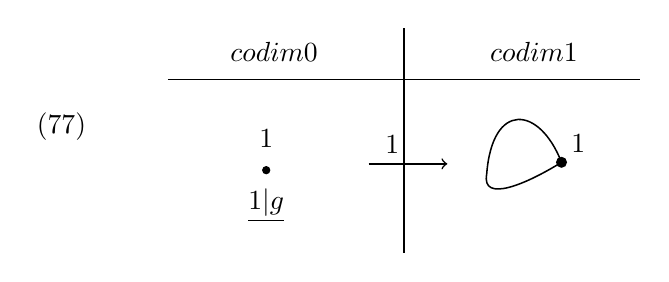
\begin{tikzpicture}[x=1cm,y=1cm,line width=.55pt]
\node at (-1.35,.55) {$(77)$};
\draw (0,1.15)--(6,1.15);
\draw (3,1.8)--(3,-1.05);
\node at (1.35,1.5) {$\text{codim }0$};
\node at (4.65,1.5) {$\text{codim }1$};
\fill (1.25,0) circle (1.5pt);
\node at (1.25,.4) {$1$};
\node at (1.25,-.45) {$\underline{\unsure{1|g}}$};
\draw[->] (2.55,.08)--(3.55,.08);
\node at (2.85,.32) {$1$};
\draw (5,.1)..controls(4.72,.82)and(4.12,.88)..(4.05,-.05)..controls(3.98,-.42)and(4.55,-.18)..(5,.1);
\fill (5,.1) circle (2pt);
\node[above right] at (5,.1) {$1$};
\end{tikzpicture}}
There is exactly one point at infinity.

We have a morphism (\uline{over} $\mathbb Z[\frac12]$)
\[
(78)\qquad \overset{\deleted{\unsure{\wedge}}}{M}_{1,1}\longrightarrow\overset{\deleted{\unsure{\wedge}}}{M}'_{1,4}\overset{\mathrm{definition}}{=}(\overset{\deleted{\unsure{\wedge}}}{M}^!_{1,4},\mathfrak S_3)
\]
which makes $\overset{\deleted{\unsure{\wedge}}}{M}_{1,1}$ a gerbe (with constant group $\{\pm1\}$) over $\overset{\deleted{\unsure{\wedge}}}{M}'_{1,4}$ (in characteristic $\neq2$)
\[
\text{hence}\qquad [M_{1,1}]=\frac12[U_{0,3},\mathfrak S_3]=\unsure{2|\frac12}[M_{0,4}]\underset{\inserted{T(1)}}{\deleted{\unsure{=\tfrac1{12}[\mathbb E^1]-\tfrac14}}}
\]
\margin{62}
